% ============================================================
%  Chapter 2: Limits of Sequences & Limits of Functions
%  Source: Tongji 8th-edition courseware (S1_2 + S1_3)
%  English Beamer lecture slides — step-by-step examples via \pause
%  Key diagrams use original PPT screenshots via \includegraphics
% ============================================================
\documentclass[aspectratio=169,10pt]{beamer}

\usetheme{Madrid}
\usecolortheme{default}
\usepackage{amsmath,amssymb,amsthm}
\usepackage{mathtools}
\usepackage{tikz}
\usetikzlibrary{shapes,arrows.meta,positioning,calc,decorations.pathreplacing}
\graphicspath{{images/}}

\title{Chapter 2: Limits}
\subtitle{Limits of Sequences \& Limits of Functions}
\author{Advanced Mathematics \\ (Tongji University, 8th Ed.)}
\date{}
\institute{}

% ------------------------------------------------------------
\begin{document}

% ==================== TITLE ====================
\begin{frame}
  \titlepage
\end{frame}

% ==================== TABLE OF CONTENTS ====================
\begin{frame}{Outline}
  \tableofcontents
\end{frame}

% ############################################################
\section{Limits of Sequences}
% ############################################################

% -------------------- Section Overview --------------------
\begin{frame}{Section 2: Limits of Sequences --- Roadmap}
  \begin{enumerate}
    \item Definition of the Limit of a Sequence
    \item Properties of Convergent Sequences
    \item Existence Criteria and Two Important Limits
  \end{enumerate}
  \vfill
  \begin{block}{Key Idea}
    A sequence $\{x_n\}$ \textbf{converges} to $a$ if its terms get
    arbitrarily close to $a$ as $n$ grows.
  \end{block}
\end{frame}

% -------------------- Motivation --------------------
\begin{frame}{Motivation: Measuring Area}
  \begin{exampleblock}{Problem}
    Find the area of a region by inscribing polygons.
  \end{exampleblock}
  \pause
  \begin{columns}
    \column{0.55\textwidth}
    \begin{itemize}
      \item<2-> True value of side length: unknown.
      \item<3-> Direct observation gives approximate values.
      \item<4-> As precision improves, approximations approach the true value.
    \end{itemize}
    \column{0.42\textwidth}
    \begin{center}
      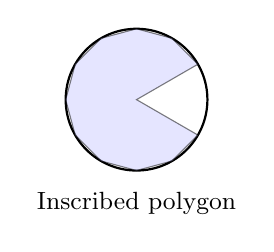
\begin{tikzpicture}[scale=0.6]
        \draw[thick] (0,0) circle (1.5);
        \draw[fill=blue!20,opacity=0.5]
          (0,0) -- (30:1.5) -- (60:1.5) -- (90:1.5) -- (120:1.5)
          -- (150:1.5) -- (180:1.5) -- (210:1.5) -- (240:1.5)
          -- (270:1.5) -- (300:1.5) -- (330:1.5) -- cycle;
        \node at (0,-2.2) {\small Inscribed polygon};
      \end{tikzpicture}
    \end{center}
  \end{columns}
\end{frame}

% -------------------- Definition of Sequence --------------------
\begin{frame}{What Is a Sequence?}
  \begin{definition}[Sequence]
    If the independent variable takes positive integer values,
    the function
    \[
      x_n = f(n),\quad n=1,2,3,\ldots
    \]
    is called a \textbf{sequence}, denoted by $\{x_n\}$.
  \end{definition}
  \pause
  \begin{block}{Terminology}
    \begin{itemize}
      \item $x_n$ is called the \textbf{general term} (or $n$-th term).
      \item The sequence is also written as $x_1,x_2,x_3,\ldots ,x_n,\ldots$
    \end{itemize}
  \end{block}
\end{frame}

% -------------------- ε-N Definition --------------------
\begin{frame}{$\varepsilon$--$N$ Definition of Limit}
  \begin{definition}[$\varepsilon$--$N$ Definition]
    Let $\{x_n\}$ be a sequence and $a$ a constant.
    If for every $\varepsilon>0$, there exists a positive integer $N$ such that
    \[
      n > N \;\Longrightarrow\; |x_n - a| < \varepsilon,
    \]
    then we say the sequence \textbf{converges} to $a$, denoted by
    \[
      \lim_{n\to\infty}x_n = a \quad\text{or}\quad x_n \to a\;(n\to\infty).
    \]
  \end{definition}
  \pause
  \begin{alertblock}{Divergence}
    If no such $a$ exists, the sequence is said to \textbf{diverge}.
  \end{alertblock}
\end{frame}

% -------------------- Geometric Interpretation (ORIGINAL IMAGE) --------------------
\begin{frame}{Geometric Interpretation of $\varepsilon$--$N$}
  \begin{center}
    \includegraphics[width=0.82\textwidth,height=0.60\textheight,keepaspectratio]{S1_2_s03.png}
  \end{center}
  \pause
  \begin{block}{Equivalent Formulation}
    \[
      \lim_{n\to\infty}x_n=a
      \quad\Longleftrightarrow\quad
      \forall\,\varepsilon>0,\;\exists\,N>0:\; n>N \Rightarrow x_n\in(a-\varepsilon,\,a+\varepsilon).
    \]
  \end{block}
\end{frame}

% -------------------- Convergence vs Divergence Examples --------------------
\begin{frame}{Convergent vs.\ Divergent Sequences}
  \begin{columns}
    \column{0.48\textwidth}
    \begin{block}{Convergent}
      \begin{itemize}
        \item $\displaystyle\frac{1}{n}\to 0$
        \item $\displaystyle\frac{n}{n+1}\to 1$
        \item $\displaystyle q^n\to 0$ \;( $|q|<1$ )
        \item $\displaystyle\frac{(-1)^n}{n}\to 0$
      \end{itemize}
    \end{block}
    \column{0.48\textwidth}
    \begin{alertblock}{Divergent}
      \begin{itemize}
        \item $(-1)^n$: oscillates
        \item $n^2\to+\infty$
        \item $(-n)\to-\infty$
        \item $1+(-1)^n/n$: bounded but not convergent
      \end{itemize}
    \end{alertblock}
  \end{columns}
  \vspace{1em}
  \pause
  \begin{center}
    \textit{Trend is definite $\Rightarrow$ convergent; trend is indefinite $\Rightarrow$ divergent.}
  \end{center}
\end{frame}

% ==================== EXAMPLES (ε-N Proofs) ====================
% -------------------- Example 1 --------------------
\begin{frame}{Example 1: $\displaystyle\lim_{n\to\infty}\frac{n+(-1)^n}{n}=1$}
  \begin{example}
    Given $x_n = \dfrac{n+(-1)^n}{n}$, prove $\displaystyle\lim_{n\to\infty}x_n = 1$.
  \end{example}
  \pause
  \begin{proof}[Proof Sketch]
    Compute:
    \[
      |x_n - 1| = \left|\frac{n+(-1)^n}{n}-1\right| = \left|\frac{(-1)^n}{n}\right| = \frac{1}{n}.
    \]
  \end{proof}
  \pause
  \begin{block}{Finding $N$}
    For any $\varepsilon>0$, we want $|x_n-1|<\varepsilon$, i.e.\ $\dfrac{1}{n}<\varepsilon$; this holds as long as $n > \dfrac{1}{\varepsilon}$.
  \end{block}
\end{frame}

\begin{frame}{Example 1 (continued)}
  \begin{block}{Conclusion}
    Take $N = \left\lfloor\dfrac{1}{\varepsilon}\right\rfloor$.
    Then whenever $n > N$,
    \[
      \left|\frac{n+(-1)^n}{n}-1\right| = \frac{1}{n} < \varepsilon.
    \]
  \end{block}
  \pause
  \begin{center}
    \Large$\displaystyle\lim_{n\to\infty}\frac{n+(-1)^n}{n}=1$ \hfill$\blacksquare$
  \end{center}
\end{frame}

% -------------------- Example 2 --------------------
\begin{frame}{Example 2: $\displaystyle\lim_{n\to\infty}\frac{(-1)^n}{(n+1)^2}=0$}
  \begin{example}
    Given $x_n = \dfrac{(-1)^n}{(n+1)^2}$, prove $\displaystyle\lim_{n\to\infty}x_n = 0$.
  \end{example}
  \pause
  \begin{proof}[Proof Sketch]
    \[
      |x_n - 0| = \left|\frac{(-1)^n}{(n+1)^2}\right|
                = \frac{1}{(n+1)^2} < \frac{1}{n+1}.
    \]
  \end{proof}
  \pause
  \begin{block}{Finding $N$}
    For any $\varepsilon\in(0,1)$, want $|x_n-0|<\varepsilon$.\\
    It suffices that $\dfrac{1}{n+1}<\varepsilon$, i.e.\ $n > \dfrac{1}{\varepsilon}-1$.
  \end{block}
\end{frame}

\begin{frame}{Example 2 (continued)}
  \begin{block}{Conclusion}
    Take $N = \left\lfloor\dfrac{1}{\varepsilon}-1\right\rfloor$.
    Then when $n > N$,
    \[
      |x_n - 0| < \varepsilon \quad\Longrightarrow\quad
      \lim_{n\to\infty}\frac{(-1)^n}{(n+1)^2}=0.
    \]
  \end{block}
  \pause
  \begin{alertblock}{Note}
    $N$ depends on $\varepsilon$ but is \textbf{not unique}.\\
    One could also take $N = \left\lfloor\dfrac{1}{\sqrt{\varepsilon}}-1\right\rfloor$ (a tighter bound).\\
    Any $N$ satisfying the condition works; it need not be the smallest.
  \end{alertblock}
\end{frame}

% -------------------- Example 3 --------------------
\begin{frame}{Example 3: $\displaystyle\lim_{n\to\infty}\frac{1}{n^\alpha}=0\;(\alpha>0)$}
  \begin{example}
    Let $\alpha > 0$. Prove $\displaystyle\lim_{n\to\infty}\frac{1}{n^\alpha}=0$.
  \end{example}
  \pause
  \begin{proof}[Proof Sketch]
    We want $\left|\dfrac{1}{n^\alpha}-0\right| = \dfrac{1}{n^\alpha} < \varepsilon$.\\[6pt]
    This is equivalent to $n^\alpha > \dfrac{1}{\varepsilon}$, i.e.\ $n > \varepsilon^{-1/\alpha}$.
  \end{proof}
  \pause
  \begin{block}{Conclusion}
    Take $N = \left\lfloor\varepsilon^{-1/\alpha}\right\rfloor$.
    Then $n > N \;\Longrightarrow\; \dfrac{1}{n^\alpha} < \varepsilon$.
    Hence $\displaystyle\lim_{n\to\infty}\frac{1}{n^\alpha}=0$.
    \hfill$\blacksquare$
  \end{block}
\end{frame}

% ==================== PROPERTIES ====================
% -------------------- Property 1: Uniqueness --------------------
\begin{frame}{Property 1: Uniqueness of the Limit}
  \begin{theorem}[Uniqueness]
    The limit of a convergent sequence is \textbf{unique}.
  \end{theorem}
  \pause
  \begin{proof}[Proof by Contradiction]
    Suppose $\displaystyle\lim_{n\to\infty}x_n = a$ and
    $\displaystyle\lim_{n\to\infty}x_n = b$ with $a \neq b$.
    \pause
    Take $\varepsilon = \dfrac{|a-b|}{2}>0$.
    \pause
    Since $x_n \to a$, $\exists\,N_1$: $n>N_1 \Rightarrow |x_n-a|<\varepsilon$.
    \pause
    Since $x_n \to b$, $\exists\,N_2$: $n>N_2 \Rightarrow |x_n-b|<\varepsilon$.
  \end{proof}
\end{frame}

\begin{frame}{Property 1 (continued)}
  \begin{proof}[Proof (cont.)]
    Let $N = \max\{N_1,N_2\}$. When $n > N$:
    \begin{align*}
      |a-b| &= |(a-x_n)+(x_n-b)| \\
            &\leq |x_n-a| + |x_n-b| \\
            &< \varepsilon + \varepsilon = 2\varepsilon = |a-b|.
    \end{align*}
    \pause
    This gives $|a-b| < |a-b|$ --- a \textbf{contradiction}!
  \end{proof}
  \pause
  \begin{center}
    Therefore the limit must be unique. \hfill$\blacksquare$
  \end{center}
\end{frame}

% -------------------- Example 4: Divergence via Uniqueness --------------------
\begin{frame}{Example 4: $x_n=(-1)^n$ Diverges}
  \begin{example}
    Prove that the sequence $x_n = (-1)^n$ diverges.
  \end{example}
  \pause
  \begin{proof}[Proof by Contradiction]
    Assume $\{x_n\}$ converges to some limit $a$.
    \pause
    Take $\varepsilon = \dfrac{1}{2}$.
    By convergence, $\exists\,N$: $n>N \Rightarrow |x_n - a| < \dfrac{1}{2}$.
    \pause
    But $x_n$ alternates between $1$ and $-1$:
    \[
      x_{2k}=1,\quad x_{2k+1}=-1.
    \]
    Both cannot lie in an interval of length $1$ centered at $a$ simultaneously.
  \end{proof}
  \pause
  \begin{center}
    Contradiction $\Rightarrow$ $\{(-1)^n\}$ \textbf{diverges}. \hfill$\blacksquare$
  \end{center}
\end{frame}

% -------------------- Property 2: Boundedness --------------------
\begin{frame}{Property 2: Convergent $\Rightarrow$ Bounded}
  \theoremstyle{definition}
  \begin{theorem}[Boundedness]
    Every convergent sequence is \textbf{bounded}.
  \end{theorem}
  \pause
  \begin{proof}
    Let $\displaystyle\lim_{n\to\infty}x_n = a$. Take $\varepsilon = 1$.
    \pause
    Then $\exists\,N$: for all $n > N$, $|x_n - a| < 1$.
    \pause
    Hence $|x_n| < |a| + 1$ for $n > N$.
    \pause
    Let $M = \max\{|x_1|,|x_2|,\ldots,|x_N|,\,|a|+1\}$.
    Then $|x_n| \leq M$ for all $n$.
  \end{proof}
  \pause
  \begin{center}
    Therefore $\{x_n\}$ is bounded. \hfill$\blacksquare$
  \end{center}
\end{frame}

\begin{frame}{Bounded $\not\Rightarrow$ Convergent!}
  \begin{alertblock}{The Converse Is False}
    Boundedness does \textbf{not} imply convergence.
  \end{alertblock}
  \pause
  \begin{example}[Counterexample]
    The sequence $x_n = (-1)^n$ is bounded ($|x_n|\leq 1$) but does \textbf{not} converge.
  \end{example}
  \pause
  \begin{center}
    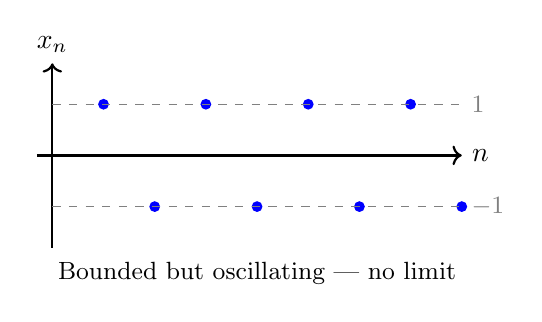
\begin{tikzpicture}[scale=0.65]
      \draw[->,thick] (-0.3,0) -- (8,0) node[right] {$n$};
      \draw[->,thick] (0,-1.8) -- (0,1.8) node[above] {$x_n$};
      \foreach \i in {0,1,...,7}{
        \pgfmathsetmacro{\y}{mod(\i,2)==0 ? 1 : -1}
        \fill[blue] (\i+1,\y) circle (3pt);
      }
      \draw[dashed,gray] (0,1) -- (8,1) node[right,font=\small] {$1$};
      \draw[dashed,gray] (0,-1) -- (8,-1) node[right,font=\small] {$-1$};
      \node at (4,-2.3) {\small Bounded but oscillating --- no limit};
    \end{tikzpicture}
  \end{center}
\end{frame}

% -------------------- Property 3: Sign-Preserving --------------------
\begin{frame}{Property 3: Local Sign-Preserving Property}
  \begin{theorem}[Sign-Preserving]
    If $\displaystyle\lim_{n\to\infty}x_n = a$ and $a > 0$ (or $a < 0$),
    then from some term onward, $x_n > 0$ (or $x_n < 0$).
  \end{theorem}
  \pause
  \begin{proof}
    Assume $a > 0$. Take $\varepsilon = \dfrac{a}{2} > 0$.
    \pause
    $\exists\,N$: for all $n > N$,
    \[
      |x_n - a| < \frac{a}{2}
      \quad\Longrightarrow\quad
      -\frac{a}{2} < x_n - a < \frac{a}{2}.
    \]
    \pause
    In particular, $x_n > a - \dfrac{a}{2} = \dfrac{a}{2} > 0$ for all $n > N$.
  \end{proof}
\end{frame}

\begin{frame}{Corollary: Strictly Positive Limit}
  \begin{corollary}
    If $\displaystyle\lim_{n\to\infty}x_n = a$ with $a > 0$,
    then there exists $N$ such that $x_n > 0$ for all $n > N$.
  \end{corollary}
  \pause
  \begin{block}{Stronger Form}
    More generally, if $a > b$, then $x_n > b$ for all sufficiently large $n$.
    (Apply the theorem to the sequence $y_n = x_n - b$.)
  \end{block}
\end{frame}

% -------------------- Property 4: Subsequences --------------------
\begin{frame}{Property 4: Subsequences Converge to the Same Limit}
  \begin{theorem}[Subsequence Convergence]
    If $\displaystyle\lim_{n\to\infty}x_n = a$, then \textbf{every subsequence}
    $\{x_{n_k}\}$ also converges to $a$.
  \end{theorem}
  \pause
  \begin{proof}
    Since $x_n \to a$: $\forall\,\varepsilon>0$, $\exists\,N$ such that
    \[
      n > N \;\Longrightarrow\; |x_n - a| < \varepsilon.
    \]
    \pause
    The subsequence indices satisfy $n_k \geq k$.
    Choose $K = N$. Then for all $k > K$:
    \[
      n_k \geq k > N \;\Longrightarrow\; |x_{n_k} - a| < \varepsilon.
    \]
  \end{proof}
  \pause
  \begin{center}
    Hence $\displaystyle\lim_{k\to\infty}x_{n_k} = a$. \hfill$\blacksquare$
  \end{center}
\end{frame}

% -------------------- Divergence via Subsequences --------------------
\begin{frame}{Using Subsequences to Prove Divergence}
  \begin{alertblock}{Practical Criterion for Divergence}
    If a sequence has two subsequences converging to \textbf{different} limits,
    then the original sequence \textbf{diverges}.
  \end{alertblock}
  \pause
  \begin{example}
    $x_n = \sin\!\left(\dfrac{n\pi}{2}\right)$:
    \begin{itemize}
      \item Subsequence $x_{4k} = \sin(2k\pi) = 0 \to 0$
      \item Subsequence $x_{4k+1} = \sin(2k\pi+\frac{\pi}{2}) = 1 \to 1$
    \end{itemize}
    Different limits $\Rightarrow$ $\{x_n\}$ diverges.
  \end{example}
\end{frame}

% ==================== EXISTENCE CRITERIA =================---
% -------------------- Overview --------------------
\begin{frame}{Existence Criteria: Overview}
  How do we know a limit exists without knowing its value?
  \vspace{0.5em}
  \pause
  \begin{enumerate}
    \item<2-> \textbf{Squeeze (Sandwich) Criterion} \hfill (p.\,46)
    \item<3-> \textbf{Monotone Bounded Sequence Criterion} \hfill (p.\,48)
    \item<4-> \textbf{Cauchy Convergence Principle} \hfill (p.\,51)\; {\small(starred)}
  \end{enumerate}
  \vfill
  \onslide<5->{
    \begin{block}{Key Insight}
      These criteria allow us to prove existence of limits
      even when the exact value is hard to compute directly.
    \end{block}
  }
\end{frame}

% -------------------- Squeeze Criterion (ORIGINAL IMAGE) --------------------
\begin{frame}{Criterion 1: Squeeze (Sandwich) Theorem}
  \begin{theorem}[Squeeze Criterion]
    Suppose sequences $\{y_n\}$, $\{x_n\}$, $\{z_n\}$ satisfy:
    \begin{enumerate}
      \item[(1)] $y_n \leq x_n \leq z_n$ \quad for $n=1,2,\ldots$
      \item[(2)] $\displaystyle\lim_{n\to\infty}y_n = \lim_{n\to\infty}z_n = a$
    \end{enumerate}
    Then $\displaystyle\lim_{n\to\infty}x_n = a$.
  \end{theorem}
  \pause
  \begin{center}
    \includegraphics[width=0.75\textwidth,height=0.45\textheight,keepaspectratio]{S1_2_s14.png}
  \end{center}
\end{frame}

% -------------------- Monotone Bounded (ORIGINAL IMAGE) --------------------
\begin{frame}{Criterion 2: Monotone Bounded Sequence}
  \begin{theorem}[Monotone Bounded Convergence]
    A monotone (increasing or decreasing) and bounded sequence
    always has a limit.
  \end{theorem}
  \pause
  \begin{center}
    \includegraphics[width=0.70\textwidth,height=0.50\textheight,keepaspectratio]{S1_2_s14.png}
  \end{center}
  \pause
  \[
    \text{Monotone } + \text{ Bounded } \quad\Longrightarrow\quad
    \lim_{n\to\infty}x_n = b \;\;(\leq M \text{ or } \geq m)
  \]
\end{frame}

% -------------------- Cauchy Criterion (starred) --------------------
\begin{frame}{*Criterion 3: Cauchy Convergence Principle}
  \begin{theorem}[Cauchy Criterion]\label{thm:cauchy}
    A sequence $\{x_n\}$ has a limit \textbf{if and only if}:
    \[
      \forall\,\varepsilon>0,\;\exists\,N>0:\;
      m,n > N \;\Longrightarrow\; |x_m - x_n| < \varepsilon.
    \]
  \end{theorem}
  \pause
  \begin{proof}[``Necessity'' ($\Rightarrow$)]
    Let $\displaystyle\lim_{n\to\infty}x_n = a$.
    \pause
    Given $\varepsilon>0$, $\exists\,N$: $n>N \Rightarrow |x_n-a|<\dfrac{\varepsilon}{2}$.
    \pause
    Then for $m,n > N$:
    \[
      |x_m-x_n| \leq |x_m-a|+|a-x_n| < \frac{\varepsilon}{2}+\frac{\varepsilon}{2}=\varepsilon.
    \]
  \end{proof}
  \pause
  \begin{block}{``Sufficiency'' ($\Leftarrow$)}
    Proof omitted (requires completeness of $\mathbb{R}$).
  \end{block}
\end{frame}

% -------------------- Summary S1_2 --------------------
\begin{frame}{Summary: Limits of Sequences}
  \begin{enumerate}
    \item \textbf{$\varepsilon$--$N$ Definition} and applications
    \item \textbf{Properties of convergent sequences}:
    \begin{itemize}
      \item Uniqueness
      \item Boundedness (converse false!)
      \item Local sign-preserving property
      \item All subsequences converge to the same limit
    \end{itemize}
    \item \textbf{Existence Criteria}:
    \begin{itemize}
      \item Squeeze (Sandwich) Criterion
      \item Monotone Bounded Criterion
      \item *Cauchy Convergence Principle
    \end{itemize}
  \end{enumerate}
\end{frame}

\begin{frame}{Think \& Exercise}
  \begin{block}{Discussion Question}
    What are the ways to show that a limit does \textbf{not} exist?
  \end{block}
  \pause
  \begin{enumerate}
    \item Find a subsequence tending to $+\infty$ or $-\infty$.
    \item Find two subsequences converging to \textbf{different} limits.
  \end{enumerate}
\end{frame}

% ############################################################
\section{Limits of Functions}
% ############################################################

% -------------------- Section Overview --------------------
\begin{frame}{Section 3: Limits of Functions --- Roadmap}
  \begin{enumerate}
    \item Limits as $x \to x_0$ (finite point)
    \item Limits as $x \to \infty$ (at infinity)
  \end{enumerate}
  \vfill
  \begin{block}{Central Question}
    What does it mean for $f(x)$ to approach a value $A$ as $x$ approaches some target?
  \end{block}
\end{frame}

% -------------------- Motivation: Precision --------------------
\begin{frame}{Motivation: Precision in Measurement}
  \begin{exampleblock}{Problem}
    Measure the area of a square by observing its side length.
  \end{exampleblock}
  \pause
  \begin{itemize}
    \item<2-> \textbf{True value}: side length $= x_0$, area $= x_0^2$.
    \item<3-> \textbf{Direct observation}: measure side $\approx x$, compute area $\approx x^2$.
    \item<4-> \textbf{Indirect observation}: want area accurate within $\varepsilon$.
  \end{itemize}
  \vspace{0.5em}
  \onslide<5->{
    \begin{block}{Key Question}
      Given any precision $\varepsilon > 0$, how close must $x$ be to $x_0$
      to guarantee $|x^2 - x_0^2| < \varepsilon$?\\[4pt]
      Answer: find $\delta > 0$ such that $|x - x_0| < \delta$ suffices.
    \end{block}
  }
\end{frame}

% -------------------- ε-δ Definition --------------------
\begin{frame}{Definition 1: $\varepsilon$--$\delta$ Definition ($x \to x_0$)}
  \begin{definition}[$\varepsilon$--$\delta$ Limit]
    Let $f(x)$ be defined in some deleted neighbourhood of $x_0$.
    If
    \[
      \forall\,\varepsilon>0,\;\exists\,\delta>0:\;
      0<|x-x_0|<\delta \;\Longrightarrow\; |f(x)-A|<\varepsilon,
    \]
    then the constant $A$ is called the \textbf{limit} of $f(x)$ as $x\to x_0$:
    \[
      \lim_{x\to x_0}f(x)=A \quad\text{or}\quad f(x)\to A\;(x\to x_0).
    \]
  \end{definition}
  \pause
  \begin{block}{Equivalent Formulation}
    \[
      \lim_{x\to x_0}f(x)=A
      \;\Longleftrightarrow\;
      \forall\,\varepsilon>0,\;\exists\,\delta>0:\;
      x\in\mathring{U}(x_0,\delta) \;\Longrightarrow\; |f(x)-A|<\varepsilon.
    \]
  \end{block}
\end{frame}

% -------------------- Geometric Interpretation ε-δ (ORIGINAL IMAGE) --------------------
\begin{frame}{Geometric Interpretation of $\varepsilon$--$\delta$}
  \begin{center}
    \includegraphics[width=0.80\textwidth,height=0.60\textheight,keepaspectratio]{S1_3_s03.png}
  \end{center}
  \pause
  \begin{block}{Immediate Consequence}
    Limit existence $\Longrightarrow$ function is \textbf{locally bounded}
    near $x_0$. \hfill(P32, Theorem 2)
  \end{block}
\end{frame}

% -------------------- Example 0: Constant Function --------------------
\begin{frame}{Example 0: $\displaystyle\lim_{x\to x_0}C = C$}
  \begin{example}
    Prove $\displaystyle\lim_{x\to x_0} C = C$ where $C$ is a constant.
  \end{example}
  \pause
  \begin{proof}[Proof]
    \[
      |f(x) - A| = |C - C| = 0 < \varepsilon
    \]
    holds for \textbf{any} $\delta > 0$, since the left-hand side is always $0$.
  \end{proof}
  \pause
  \begin{center}
    Hence $\displaystyle\lim_{x\to x_0} C = C$. \hfill$\blacksquare$
  \end{center}
\end{frame}

% -------------------- Example 1: Basic ε-δ --------------------
\begin{frame}{Example 1: A Basic $\varepsilon$--$\delta$ Proof}
  \begin{example}
    Prove $\displaystyle\lim_{x\to x_0}x^2 = x_0^2$ using the $\varepsilon$--$\delta$ definition.
  \end{example}
  \pause
  \begin{proof}[Proof Sketch]
    \[
      |f(x)-A| = |x^2 - x_0^2| = |x-x_0|\cdot|x+x_0|.
    \]
    \pause
    Restrict $|x-x_0|<1$, so $|x|<|x_0|+1$ and $|x+x_0|<2|x_0|+1$.
    \pause
    Then $|x^2-x_0^2| < (2|x_0|+1)\cdot|x-x_0|$.
  \end{proof}
  \pause
  \begin{block}{Choosing $\delta$}
    For given $\varepsilon>0$, take $\delta = \min\left\{1,\; \dfrac{\varepsilon}{2|x_0|+1}\right\}$.\\[4pt]
    Then $0<|x-x_0|<\delta \;\Longrightarrow\; |x^2-x_0^2|<\varepsilon$. \hfill$\blacksquare$
  \end{block}
\end{frame}

% -------------------- Example 2: Linear Function --------------------
\begin{frame}{Example 2: $\displaystyle\lim_{x\to 1}(2x-1)=1$}
  \begin{example}
    Prove $\displaystyle\lim_{x\to 1}(2x-1)=1$.
  \end{example}
  \pause
  \begin{proof}[Proof]
    \[
      |f(x)-A| = |(2x-1)-1| = 2|x-1|.
    \]
    For any $\varepsilon>0$, we want $|f(x)-A|<\varepsilon$.\\[4pt]
    This holds as long as $|x-1| < \dfrac{\varepsilon}{2}$.
  \end{proof}
\end{frame}

\begin{frame}{Example 2 (continued)}
  \begin{block}{Conclusion}
    Take $\delta = \dfrac{\varepsilon}{2}$.
    Then when $0<|x-1|<\delta$:
    \[
      |f(x)-A| = |(2x-1)-1| < \varepsilon.
    \]
    Therefore $\displaystyle\lim_{x\to 1}(2x-1)=1$. \hfill$\blacksquare$
  \end{block}
\end{frame}

% -------------------- Example 3: Root Function --------------------
\begin{frame}{Example 3: $\displaystyle\lim_{x\to x_0}\sqrt{x}=\sqrt{x_0}$\;($x_0>0$)}
  \begin{example}
    Prove $\displaystyle\lim_{x\to x_0}\sqrt{x}=\sqrt{x_0}$ for $x_0>0$.
  \end{example}
  \pause
  \begin{proof}[Proof Sketch]
    \[
      |\sqrt{x}-\sqrt{x_0}| = \frac{|x-x_0|}{\sqrt{x}+\sqrt{x_0}}
      \leq \frac{|x-x_0|}{\sqrt{x_0}}.
    \]
  \end{proof}
  \pause
  \begin{block}{Choosing $\delta$}
    For any $\varepsilon>0$, take $\delta = \varepsilon\sqrt{x_0}$.\\[4pt]
    Then $0<|x-x_0|<\delta$ implies $|\sqrt{x}-\sqrt{x_0}| < \varepsilon$.\\[4pt]
    Hence $\displaystyle\lim_{x\to x_0}\sqrt{x}=\sqrt{x_0}$. \hfill$\blacksquare$
  \end{block}
\end{frame}

% -------------------- Example 4: Absolute Value / Two-Sided --------------------
\begin{frame}{Example 4: Two-Sided Limit with Absolute Value}
  \begin{example}
    Prove $\displaystyle\lim_{x\to 0}x\sin\frac{1}{x}=0$.
  \end{example}
  \pause
  \begin{proof}[Proof]
    We have
    \[
      \left|x\sin\frac{1}{x}-0\right| = |x|\cdot\left|\sin\frac{1}{x}\right| \leq |x|.
    \]
    \pause
    For any $\varepsilon>0$, take $\delta = \varepsilon$.
    \pause
    Then when $0<|x-0|<\delta$:
    \[
      \left|x\sin\frac{1}{x}\right| \leq |x| < \delta = \varepsilon.
    \]
  \end{proof}
  \pause
  \begin{center}
    Therefore $\displaystyle\lim_{x\to 0}x\sin\frac{1}{x}=0$. \hfill$\blacksquare$
  \end{center}
\end{frame}

% ==================== PROPERTIES OF FUNCTION LIMITS ====%
% -------------------- Sign-Preserving Theorem --------------------
\begin{frame}{Theorem 1: Local Sign-Preserving Property}
  \begin{theorem}[Local Sign-Preserving]\label{thm:sign-preserve}
    If $\displaystyle\lim_{x\to x_0}f(x)=A$ and $A>0$ (resp.\ $A<0$),
    then there exists a neighbourhood of $x_0$ where $f(x)>0$ (resp.\ $f(x)<0$).
  \end{theorem}
  \pause
  \begin{proof}
    Given $A>0$, take $\varepsilon = \dfrac{A}{2}>0$.
    \pause
    By the limit definition, $\exists\,\delta>0$:
    \[
      0<|x-x_0|<\delta \;\Longrightarrow\; |f(x)-A|<\frac{A}{2}.
    \]
    \pause
    Hence $f(x) > A - \dfrac{A}{2} = \dfrac{A}{2} > 0$ in $\mathring{U}(x_0,\delta)$.
  \end{proof}
\end{frame}

\begin{frame}{Corollary: Local Boundedness}
  \begin{corollary}
    If $\displaystyle\lim_{x\to x_0}f(x)=A$, then $f(x)$ is
    \textbf{locally bounded} near $x_0$.
  \end{corollary}
  \pause
  \begin{proof}
    Take $\varepsilon = 1$. $\exists\,\delta>0$:
    \[
      0<|x-x_0|<\delta \;\Longrightarrow\; |f(x)-A|<1
      \;\Longrightarrow\; |f(x)|<|A|+1.
    \]
    Set $M=|A|+1$. Then $|f(x)|\leq M$ for $x\in\mathring{U}(x_0,\delta)$.
  \end{proof}
  \hfill(P32, Corollary)
\end{frame}

% -------------------- Order-Preserving (Monotonicity) --------------------
\begin{frame}{Theorem 2: Order-Preserving Property}
  \begin{theorem}[Order-Preserving]
    If in some deleted neighbourhood of $x_0$:
    \[
      f(x) \geq g(x) \quad\text{and}\quad
      \lim_{x\to x_0}f(x)=A,\; \lim_{x\to x_0}g(x)=B,
    \]
    then $A \geq B$.
  \end{theorem}
  \pause
  \begin{proof}[Proof by Contradiction]
    Assume $A < B$. Set $h(x)=f(x)-g(x)\geq 0$ near $x_0$.
    \pause
    Then $\displaystyle\lim_{x\to x_0}h(x)=A-B<0$.
    \pause
    By Theorem~\ref{thm:sign-preserve} (sign-preserving), $h(x)<0$ near $x_0$ ---
    contradicting $h(x)\geq 0$.
  \end{proof}
  \pause
  \begin{center}
    Hence $A \geq B$. \hfill$\blacksquare$
  \end{center}
\end{frame}

\begin{frame}{Remark on Strict Inequality}
  \begin{alertblock}{Caution}
    If the condition is changed to $f(x) > g(x)$ (strict), we can only conclude
    $A \geq B$, \textbf{not necessarily} $A > B$.
  \end{alertblock}
  \pause
    \begin{example}[Counterexample]
      $f(x)=x^2$, $g(x)=0$ for all $x\neq 0$.
      Clearly $f(x)>g(x)$ for $x\neq 0$, but
      $\displaystyle\lim_{x\to 0}f(x)=\lim_{x\to 0}g(x)=0$.
    \end{example}
\end{frame}

% -------------------- Left & Right Limits --------------------
\begin{frame}{Left Limit and Right Limit}
  \begin{definition}[Left Limit]
    \[
      f(x_0^-)=\lim_{x\to x_0^-}f(x)=A
      \;\Longleftrightarrow\;
      \forall\,\varepsilon>0,\;\exists\,\delta>0:\;
      x\in(x_0-\delta,x_0) \;\Longrightarrow\; |f(x)-A|<\varepsilon.
    \]
  \end{definition}
  \pause
  \begin{definition}[Right Limit]
    \[
      f(x_0^+)=\lim_{x\to x_0^+}f(x)=A
      \;\Longleftrightarrow\;
      \forall\,\varepsilon>0,\;\exists\,\delta>0:\;
      x\in(x_0,x_0+\delta) \;\Longrightarrow\; |f(x)-A|<\varepsilon.
    \]
  \end{definition}
\end{frame}

\begin{frame}{Theorem 3: Equivalence of Two-Sided and One-Sided Limits}
  \begin{theorem}[L/R Equivalence]\label{thm:lr-equiv}
    \[
      \lim_{x\to x_0}f(x)=A
      \;\Longleftrightarrow\;
      \lim_{x\to x_0^+}f(x)=\lim_{x\to x_0^-}f(x)=A.
    \]
  \end{theorem}
  \hfill(P30)
  \vspace{1em}
  \pause
  \begin{block}{Practical Use}
    To check whether $\displaystyle\lim_{x\to x_0}f(x)$ exists:
    \begin{enumerate}
      \item Compute left limit $f(x_0^-)$.
      \item Compute right limit $f(x_0^+)$.
      \item If equal $\Rightarrow$ limit exists and equals that value.
      \item If not equal $\Rightarrow$ limit does \textbf{not} exist.
    \end{enumerate}
  \end{block}
\end{frame}

% -------------------- Example 5: Discussing Existence --------------------
\begin{frame}{Example 5: Does the Limit Exist?}
  \begin{example}
    Let $f(x)=\begin{cases} x+1, & x<0 \\ x^2, & x\geq 0 \end{cases}$.
    Discuss whether $\displaystyle\lim_{x\to 0}f(x)$ exists.
  \end{example}
  \pause
  \begin{proof}[Solution]
    Use Theorem~\ref{thm:lr-equiv} (L/R equivalence).
    \pause
    \textbf{Right limit:}
    \[
      f(0^+) = \lim_{x\to 0^+}x^2 = 0.
    \]
    \pause
    \textbf{Left limit:}
    \[
      f(0^-) = \lim_{x\to 0^-}(x+1) = 1.
    \]
  \end{proof}
\end{frame}

\begin{frame}{Example 5 (continued)}
  \begin{block}{Conclusion}
    Since $f(0^+)=0 \neq 1=f(0^-)$, the left and right limits differ.
  \end{block}
  \pause
  \begin{center}
    \Large$\displaystyle\lim_{x\to 0}f(x)$ \textbf{does NOT exist.} \hfill$\blacksquare$
  \end{center}
  \vspace{1em}
  \pause
  \begin{center}
    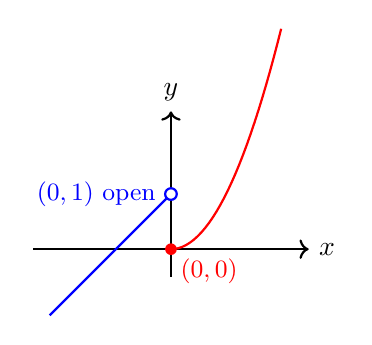
\begin{tikzpicture}[scale=0.7]
      \draw[->,thick] (-2.5,0) -- (2.5,0) node[right] {$x$};
      \draw[->,thick] (0,-0.5) -- (0,2.5) node[above] {$y$};
      % left branch: x+1 for x<0
      \draw[blue,thick,domain=-2.2:-0.05,samples=30] plot (\x, {\x+1});
      % right branch: x^2 for x>=0
      \draw[red,thick,domain=0:2,samples=30] plot (\x, {\x*\x});
      % points
      \fill[white] (0,1) circle (3pt);
      \draw[blue,thick] (0,1) circle (3pt);
      \fill[red] (0,0) circle (3pt);
      \node[blue,left] at (-0.1,1) {\small $(0,1)$ open};
      \node[red,below right] at (0,0) {\small $(0,0)$};
    \end{tikzpicture}
  \end{center}
\end{frame}

% ==================== X → ∞ LIMITS ====================
% -------------------- Definition: x → ∞ --------------------
\begin{frame}{Definition 2: Limit as $x\to\infty$}
  \begin{definition}[$x\to\infty$ Limit]
    Let $f(x)$ be defined for $|x|$ greater than some positive number.
    If
    \[
      \forall\,\varepsilon>0,\;\exists\,X>0:\;
      |x|>X \;\Longrightarrow\; |f(x)-A|<\varepsilon,
    \]
    then $A$ is the limit of $f(x)$ as $x\to\infty$:
    \[
      \lim_{x\to\infty}f(x)=A \quad\text{or}\quad f(x)\to A\;(x\to\infty).
    \]
  \end{definition}
  \pause
  \begin{block}{Equivalent Formulation}
    \[
      x<-X \;\text{ or }\; x>X \quad\Longleftrightarrow\quad
      A-\varepsilon < f(x) < A+\varepsilon.
    \]
  \end{block}
\end{frame}

% -------------------- Geometric: Horizontal Asymptote (ORIGINAL IMAGE) --------------------
\begin{frame}{Geometric Meaning: Horizontal Asymptote}
  \begin{center}
    \includegraphics[width=0.82\textwidth,height=0.60\textheight,keepaspectratio]{S1_3_s13.png}
  \end{center}
  \pause
  \begin{block}{Horizontal Asymptote}
    The line $y=A$ is a \textbf{horizontal asymptote} of the curve $y=f(x)$
    if $\displaystyle\lim_{x\to\infty}f(x)=A$ (or $x\to\pm\infty$).
  \end{block}
\end{frame}

% -------------------- Special Cases: +∞ and -∞ --------------------
\begin{frame}{Special Cases: $x\to+\infty$ and $x\to-\infty$}
  \begin{definition}[$x\to+\infty$]
    \[
      \lim_{x\to+\infty}f(x)=A
      \;\Longleftrightarrow\;
      \forall\,\varepsilon>0,\;\exists\,X>0:\;
      x>X \;\Longrightarrow\; |f(x)-A|<\varepsilon.
    \]
  \end{definition}
  \pause
  \begin{definition}[$x\to-\infty$]
    \[
      \lim_{x\to-\infty}f(x)=A
      \;\Longleftrightarrow\;
      \forall\,\varepsilon>0,\;\exists\,X>0:\;
      x<-X \;\Longrightarrow\; |f(x)-A|<\varepsilon.
    \]
  \end{definition}
  \pause
  \begin{block}{Geometric Meaning}
    In both cases, $y=A$ remains a \textbf{horizontal asymptote} of $y=f(x)$.
  \end{block}
\end{frame}

% -------------------- Example 6: 1/x → 0 --------------------
\begin{frame}{Example 6: $\displaystyle\lim_{x\to\infty}\frac{1}{x}=0$}
  \begin{example}
    Prove $\displaystyle\lim_{x\to\infty}\frac{1}{x}=0$.
  \end{example}
  \pause
  \begin{proof}[Proof]
    \[
      \left|\frac{1}{x}-0\right| = \frac{1}{|x|}.
    \]
    \pause
    For any $\varepsilon>0$, we want $\dfrac{1}{|x|}<\varepsilon$, i.e.\ $|x|>\dfrac{1}{\varepsilon}$.
    \pause
    Take $X = \dfrac{1}{\varepsilon}$.
    Then $|x|>X$ implies $\left|\dfrac{1}{x}\right|<\varepsilon$.
  \end{proof}
  \pause
  \begin{center}
    Hence $\displaystyle\lim_{x\to\infty}\frac{1}{x}=0$. \hfill$\blacksquare$
  \end{center}
\end{frame}

\begin{frame}{Example 6 (continued): Special Cases}
  \begin{alertblock}{Note}
    Similarly:
    \[
      \lim_{x\to+\infty}\frac{1}{x}=0
      \qquad\text{and}\qquad
      \lim_{x\to-\infty}\frac{1}{x}=0.
    \]
  \end{alertblock}
\end{frame}

% -------------------- Horizontal Asymptote Examples (ORIGINAL IMAGE) --------------------
\begin{frame}{Examples of Horizontal Asymptotes}
  \begin{columns}
    \column{0.48\textwidth}
    \begin{example}[Asymptote $y=0$]
      \begin{itemize}
        \item $f(x)=\dfrac{1}{\sqrt{x}}$ \;$\xrightarrow[x\to+\infty]{}\;0$
        \item $g(x)=\dfrac{1}{\sqrt{1-x}}$ \;$\xrightarrow[x\to-\infty]{}\;0$
      \end{itemize}
      Both have horizontal asymptote $y=0$.
    \end{example}
    \column{0.48\textwidth}
    \begin{example}[Asymptote $y=1$]
      \begin{itemize}
        \item $f(x)=1-2^{-x}$ \;$\xrightarrow[x\to+\infty]{}\;1$
        \item $g(x)=1+2^{x}$ \;$\xrightarrow[x\to-\infty]{}\;1$
      \end{itemize}
      Both have horizontal asymptote $y=1$.
    \end{example}
  \end{columns}
\end{frame}

\begin{frame}{Graphs of Horizontal Asymptotes}
  \begin{center}
    \includegraphics[width=0.75\textwidth,height=0.60\textheight,keepaspectratio]{S1_3_s15.png}
  \end{center}
\end{frame}

% -------------------- Summary S1_3 --------------------
\begin{frame}{Summary: Limits of Functions}
  \begin{enumerate}
    \item \textbf{$\varepsilon$--$\delta$ / $\varepsilon$--$X$ Definitions}
    \begin{itemize}
      \item $x\to x_0$: $\forall\varepsilon>0,\;\exists\delta>0:\;0<|x-x_0|<\delta\Rightarrow|f(x)-A|<\varepsilon$
      \item $x\to\infty$: $\forall\varepsilon>0,\;\exists X>0:\;|x|>X\Rightarrow|f(x)-A|<\varepsilon$
    \end{itemize}
    \item \textbf{Properties}:
    \begin{itemize}
      \item Uniqueness
      \item Local boundedness
      \item Local sign-preserving
      \item Order-preserving (monotonicity)
      \item L/R limit equivalence
    \end{itemize}
    \item \textbf{Horizontal asymptote}: $y=A$ if $\lim_{x\to\pm\infty}f(x)=A$
  \end{enumerate}
\end{frame}

\begin{frame}{Think \& Exercise}
  \begin{block}{Question 1}
    If $\displaystyle\lim_{x\to x_0}f(x)$ exists, is $f(x)$ necessarily defined at $x=x_0$?
  \end{block}
  \pause
  \begin{block}{Question 2}
    Let $f(x)$ and $g(x)$ both have limits as $x\to x_0$.
    Does $\displaystyle\lim_{x\to x_0}[f(x)\cdot g(x)]$ necessarily exist?
  \end{block}
\end{frame}

\end{document}
